%*******************************************************************************
%****************************** Fourth Chapter *********************************
%*******************************************************************************

\chapter{Results}

\ifpdf
    \graphicspath{{Chapter6/Figs/Raster/}{Chapter6/Figs/PDF/}{Chapter6/Figs/}}
\else
    \graphicspath{{Chapter6/Figs/Vector/}{Chapter6/Figs/}}
\fi

%********************************** %First Section  **************************************
\section{Image modification}

\subsection{zMod}

\begin{figure}[htbp!]
\centering
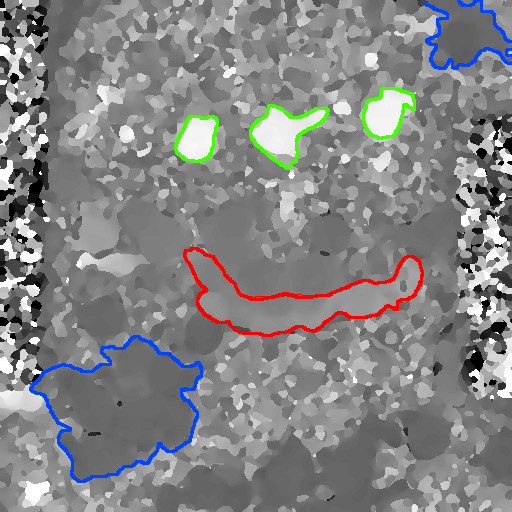
\includegraphics[width=1.0\textwidth]{5111-zmod_example_outline-050714_s13_ch-zmod-8-3-3_t0_z00}
\caption[zMod example]{An example of the zMod result.}
\label{fig:zmod_result}
\end{figure}

Although the cell outlines are not clearly visible, regions that contain cells have very uniform z-locations. Even regions outside the cells have assigned z-locations; this includes background noise and the even lower levels of background noise found in the PDMS pillars. An example is shown in Figure~\ref{fig:zmod_result}. Groups of cells at a low level are outlined in blue, mid level cells adjacent to the barrier in red, and high level cells in green.

It should be noted that this image does not indicate anything about the absolute intensity of the GFP or the Brightfield.

It's clear that there are two types of background noise: the environment and the PDMS pillars. The zMod values inside the pillars are more highly variable.

Regions of similar level are quite contiguous, even in the background. This indicates a certain amount of smoothing of the GFP (R=3, sigma=3). Smoothing was done with a Gaussian filter. The smoothing also causes the gradual transitions between adjacent regions of similar levels.

The three bright blobs at the top of the image represent three cells that lie at a high z-level in the image. At the bottom of the image, the very dark regions indicate a collection of cells that lie very low in the z-dimension of the 3D environment. It should be noted that some cells in the barrier have higher intensity than the cells below the barrier. There is a ring of lighter cancer cells in the middle. They are attached to the barrier.

This image does not indicate whether any cells overlap. It also does not reveal detailed protrusions or clear boundaries of individual cells.

\begin{figure}[htbp!]
\centering
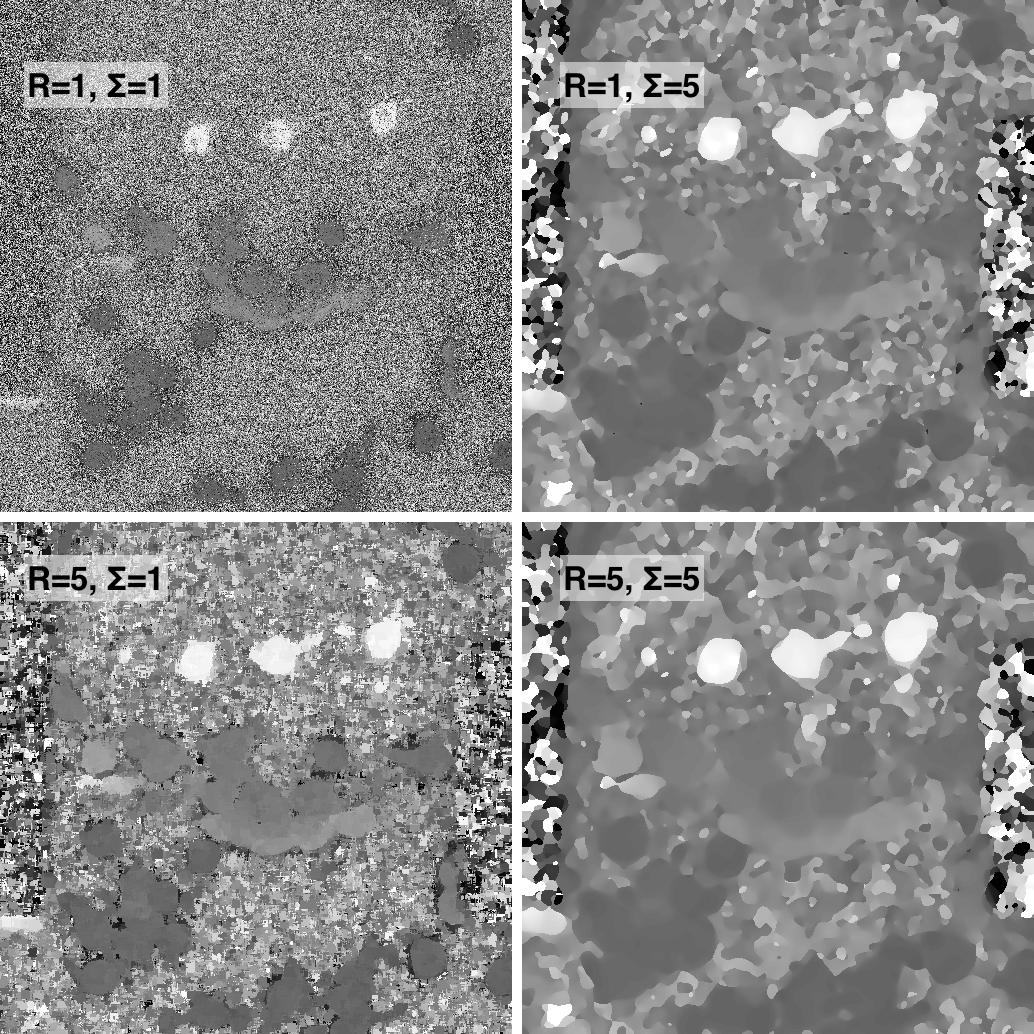
\includegraphics[width=1.0\textwidth]{5-combined_R_sigma}
\caption{The extremes of R and $\Sigma$}
\label{fig:r_and_sigma}
\end{figure}

The two main parameters that we can vary are R and Sigma. The maximum values and their results are shown in Figure~\ref{fig:r_and_sigma}.

R indicates the size of the mask used to search around the x-y position of a pixel for GFP information to use in estimating the z-position of that pixel. If R=1, only information immediately in that pixel is used to make that decision and thus the z-levels of neighbouring GFP profiles do not affect each other.

If R=5, an 11-by-11 square of pixels profiles centred on the x-y position produces the final estimate of z. This can lead to larger contiguous regions sharing similar z-values. It is worth noting that smoothing or "mixing" of z-levels occurs in 3D. Since information from every profile inside the mask is taken into account, intensities at all levels will contribute to the estimate of the z-value.

Sigma is the size of the Gaussian kernel used to smooth the GFP in 2D. The smoothing is performed before GFP profiles are generated and analysed. Since the smoothing is performed in 2D, cells that exist at very different levels in z but close proximity in x-y will not affect the profiles in each other's pixels during smoothing. If Sigma=1, little smoothing is performed and the image is very noisy. The z-levels of the pixels inside the cells are less uniform. The cells are grainy. If R=5 and Sigma=1, an effect similar to aliasing is visible [ref]. This is because of the discrete size of the mask set by R. It still appears noisy, but the effects of the noise have been spread out and diminished.

As R increases, the continuous area of the cell becomes more uniform. It is however still noisy. As Sigma increases, the effect of noise is diminished. This is because increasing R does not decrease the noise, it simply distributes its effects more widely within a mask, which has an averaging effect on a cell interior. On the other hand, increasing Sigma does actually reduce the absolute level of noise.

If Sigma=1, then the transitions between z-levels are sharper. The noise in the GFP will have a larger effect on the selection of the z-level if the GFP is not smoothed. If Sigma=5, then there is a large amount of smoothing, and noise is greatly reduced, producing more gentler transitions between parts of the same cell.

\subsection{zBF}

\begin{figure}[htbp!]
\centering
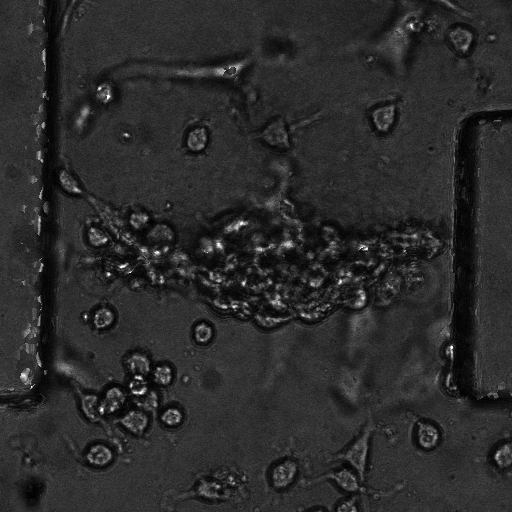
\includegraphics[width=1.0\textwidth]{5121-zbf_example-050714_s13_ch-zbf-8-3-3_t0_z00}
\caption{An example of zBF.}
\label{fig:zbf_example}
\end{figure}

As seen in Figure~\ref{fig:zbf_example}, all cells previously marked with GFP are now in focus, regardless of their z-level in the 3d environment. Delta-z has been adjusted manually to optimise the features of the cells for segmentation, i.e. where the Brightfield edges are as dark as possible and the Brightfield cell interiors are as uniform as possible. If delta-z were chosen to be higher or lower, the entire environment would appear slightly out of focus. The interiors of the cells are often non-uniform but have a higher intensity than the background. Some protrusions can clearly be seen, but others have been hidden or appear closer to the intensity of the background because they did not contain enough GFP to be adjusted by zMod properly.

The intensities in the background (notably the pillars) are highly randomised. This is due to the highly random nature of zMod in these regions but it does not directly affect the segmentation of the cancer cells.

There are some cells that appear out-of-focus such as within, above, and below the barrier. This is because they were not initially marked with GFP, so the z-position that zMod assigns to them is fairly arbitrary. The intensity profiles of these pixels are very flat, so even a small variation due to noise will cause a maximum in z to be located randomly.

\subsection{zEdge}

\begin{figure}[htbp!]
\centering
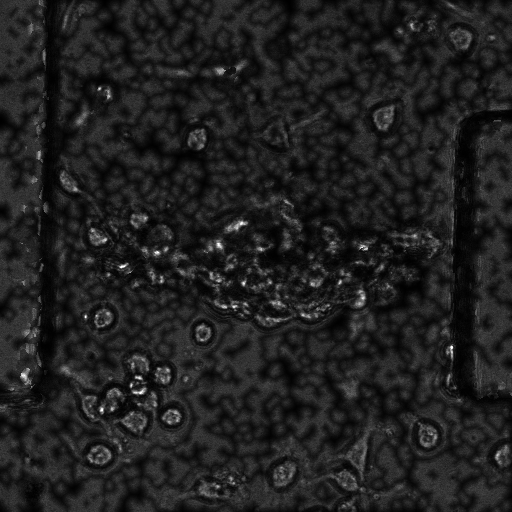
\includegraphics[width=1.0\textwidth]{5122-zedge_example-050714_s13_ch-zedge-8-3-3_t0_z00}
\caption{An example of zEdge}
\label{fig:zedge_example}
\end{figure}

The edges drawn on zEdge are similar to the Brightfield cell boundaries but are more distinct and regular, shown in Figure~\ref{fig:zedge_example}. These edges closely approximate the true boundaries of the cells. They are also better defined, which will prevent the segmentation from spilling over into the background. The edges drawn in the background are highly randomised, but this will have no effect on segmentation because there are no markers in the background.

%********************************** %Second Section  **************************************
\section{Segmentation}

\subsection{Segmentation results}

\begin{figure}[htbp!]
\centering
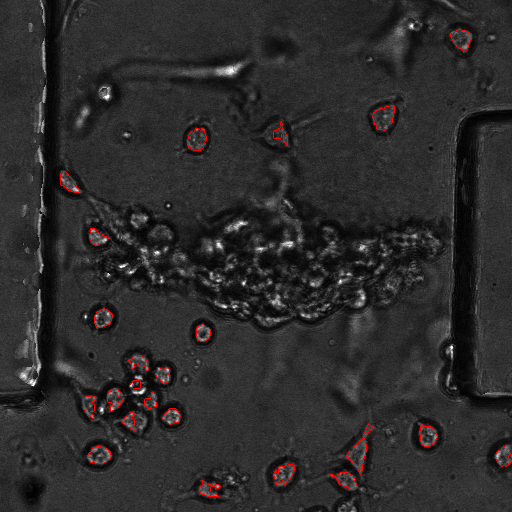
\includegraphics[width=1.0\textwidth]{5224-zedge_seg-tile_050714_s13_ch-zbf-8-5-5-outline-zcomp-8-1-1-zedge-8-5-5-TYOGE5XI_t0}
\caption{zEdge segmentation}
\label{fig:zedge_segmentation}
\end{figure}

Most of the segmentation results, shown in Figure~\ref{fig:zedge_segmentation}, very closely match the dark edges of the Brightfield. Some of the segmentation fails, especially when the interior of the cell is very non-uniform. In the bottom left of Figure~\ref{fig:zedge_segmentation}, there is a cluster of cells, in which there is a cell at the centre of this cluster for which segmentation has failed. The protrusions are not very well recognised, either because zEdge is limiting the protrusions or the protrusions are not distinct enough from the background because of the lack of GFP within them.

\begin{figure}[htbp!]
\centering
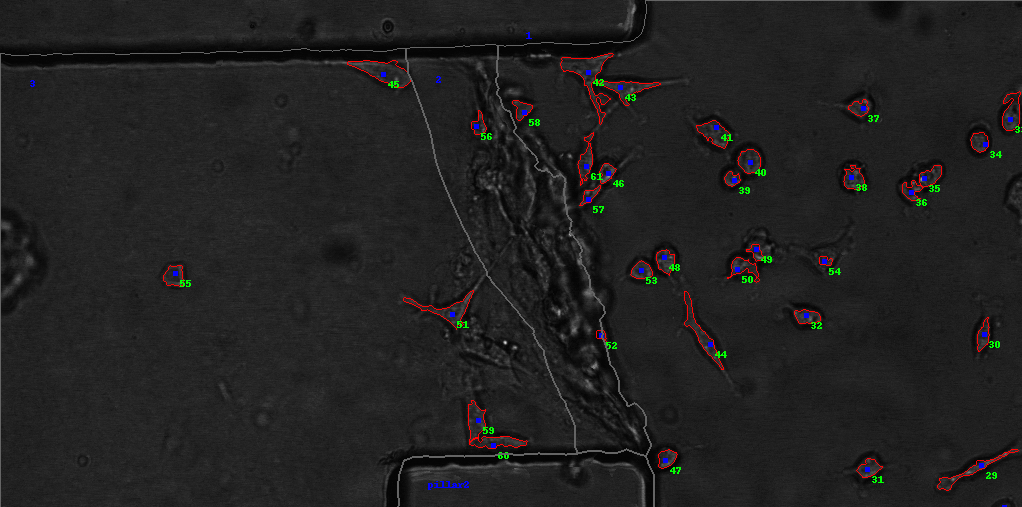
\includegraphics[width=1.0\textwidth]{good_protrusions-tile_260714_s14_t016}
\caption{Accurately segmented protrusions using zEdge.}
\label{fig:accurate_zedge}
\end{figure}

Figure~\ref{fig:accurate_zedge}, taken from another experiment from which we gathered data, is included for illustrative purposes. In this series, the cell protrusions contain more GFP and extend further from the cells. This image showcases the results of applying the zMod method more clearly in terms of protrusions. Particularly noteworthy are Cells 43, 44, and 51, whose recognitions extend very far into their protrusions with no spillover effects. Admittedly, the protrusions are still longer than the segmentation results, due to the boundaries imposed by zEdge.

\subsection{Fscore comparison}

\subsubsection{Manual ground truth}

\begin{figure}[htbp!]
\centering
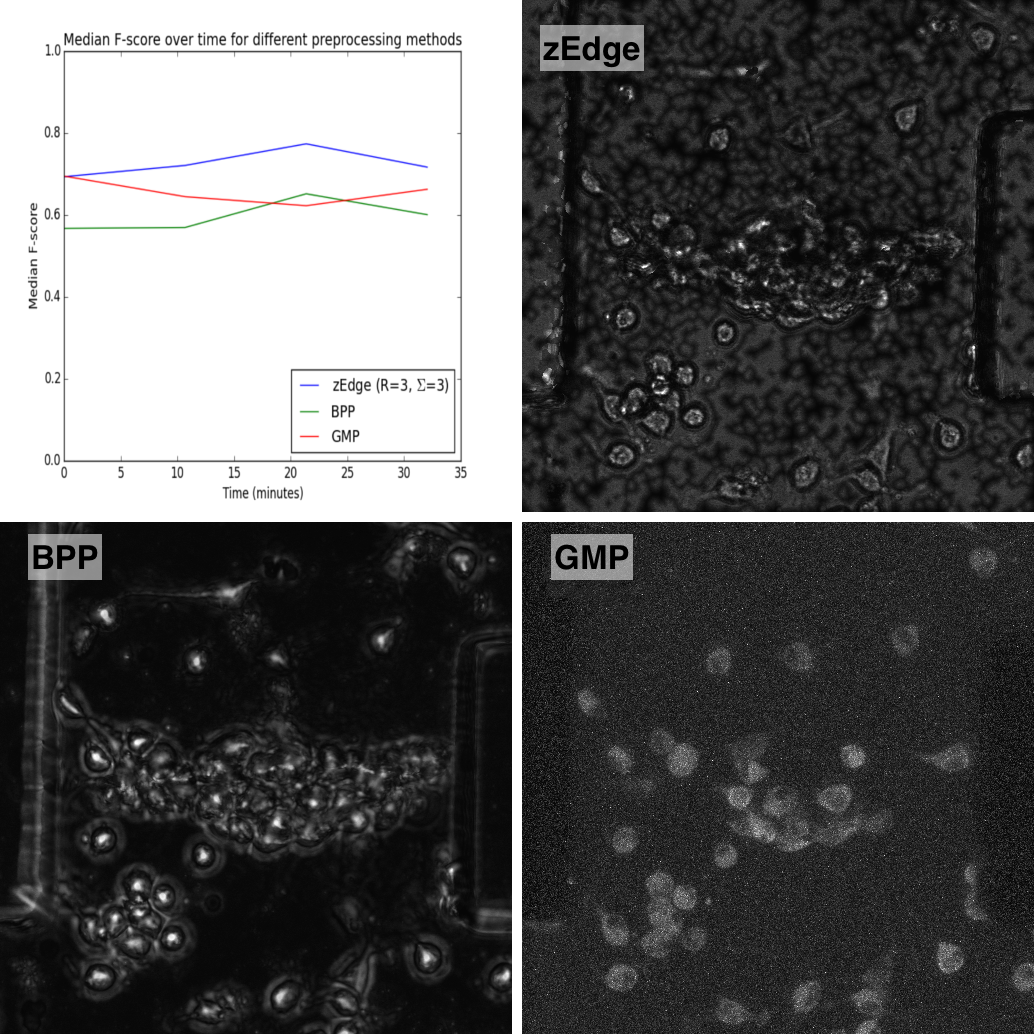
\includegraphics[width=1.0\textwidth]{6211-fscore_manual-GT_zmod_r3_s3-gmod-bmod}
\caption{Manual ground truth results}
\label{fig:manual_ground}
\end{figure}

In Figure~\ref{fig:manual_ground}, we take the result of manual segmentation to be the ground truth. The line labelled zMod represents the results of the method we propose. The line labelled bMod represents the results of the method used by Selinummi et al. The line labelled gMod represents the result of the segmentation of the GFP maximum, in which the maximum of each 3D profile in z is selected as the value for that 2D x-y position. gMod is used as ground truth in the paper by Selinummi et al.

All three of the Fscore values over time stay quite consistent. zMod has a greater median value than that of either gMod (Selinummi's ground truth) or bMod (their test method).

\subsubsection{Fluorescence ground truth}

\begin{figure}[htbp!]
\centering
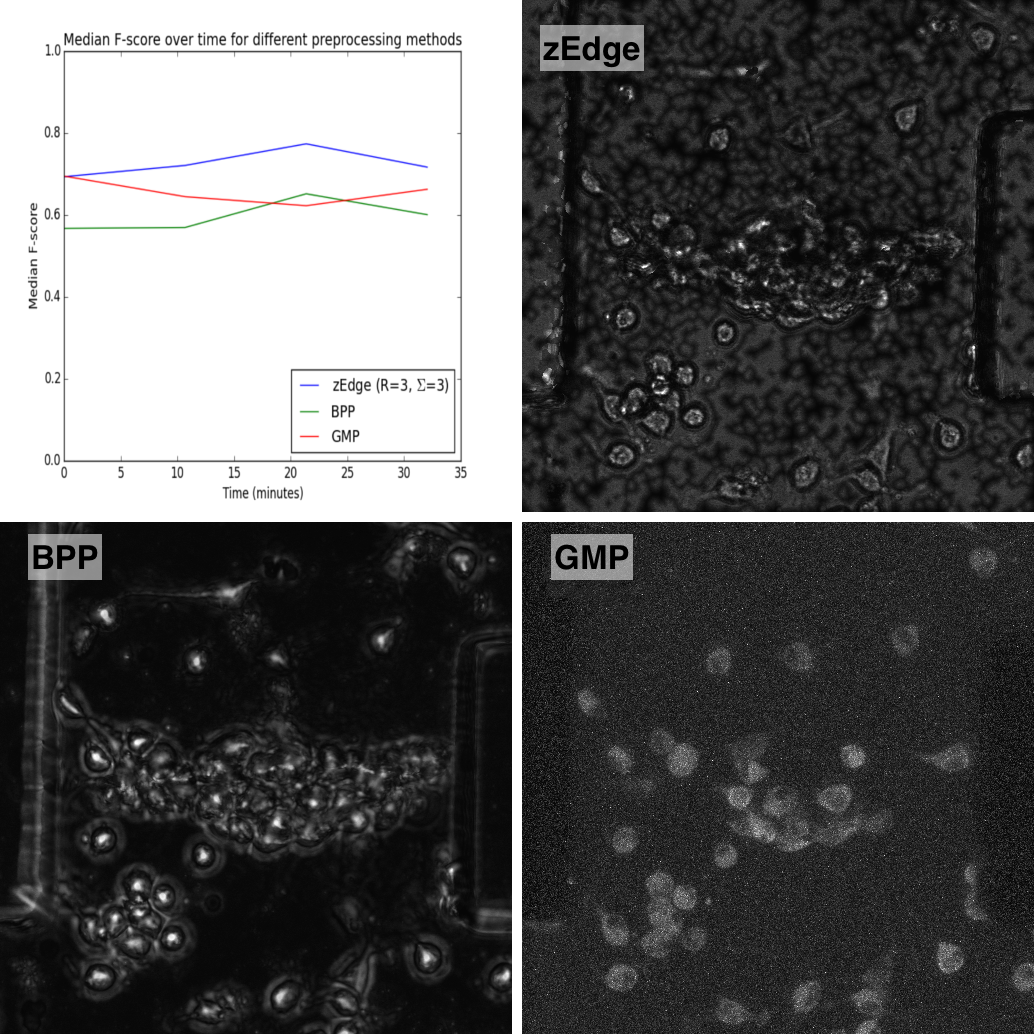
\includegraphics[width=1.0\textwidth]{6211-fscore_manual-GT_zmod_r3_s3-gmod-bmod}
\caption{GFP maximum projection segmentation}
\label{fig:gfp_maximum}
\end{figure}

In Figure~\ref{fig:gfp_maximum}, both of the methods zMod and bMod, with reference to maximum fluorescence levels used as ground truth (as seen in the Selinummi paper), have very constant median Fscores. The zMod Fscore is above the bMod Fscore.

\subsection{zMod sensitivity analysis}

\begin{figure}[htbp!]
\centering
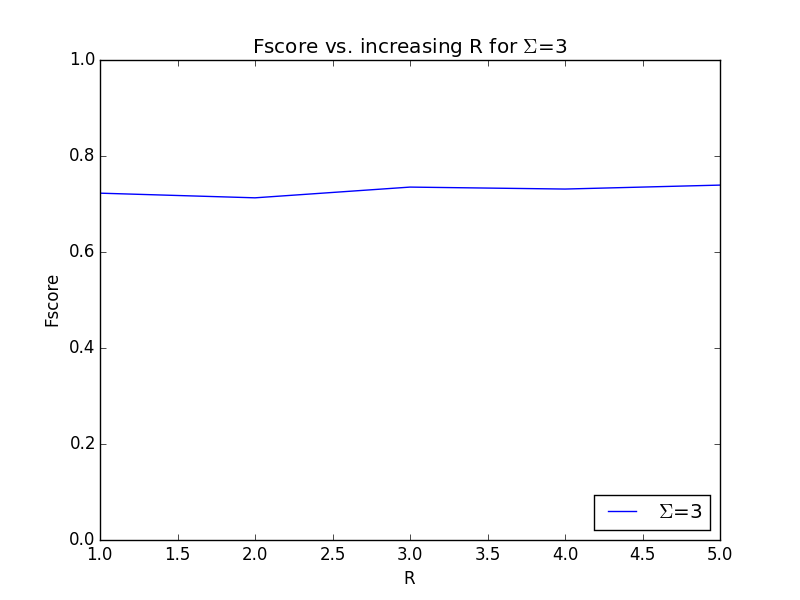
\includegraphics[width=1.0\textwidth]{6213-fscore_R_for_sigma3}
\caption{Fscore results for increasing R at constant $\Sigma=3$}
\label{fig:fscore_sigma3}
\end{figure}

The Fscore for our method, zMod, does not vary significantly with increasing R, as shown in Figure~\ref{fig:fscore_sigma3}. This means that the quality of the segmentation, using standard values for segmentation parameters, is independent of the R-value or the size of the mask linearly mixing the z-values. This would not necessarily be the case with large numbers of cells that overlapped in the z-dimension.

\begin{figure}[htbp!]
\centering
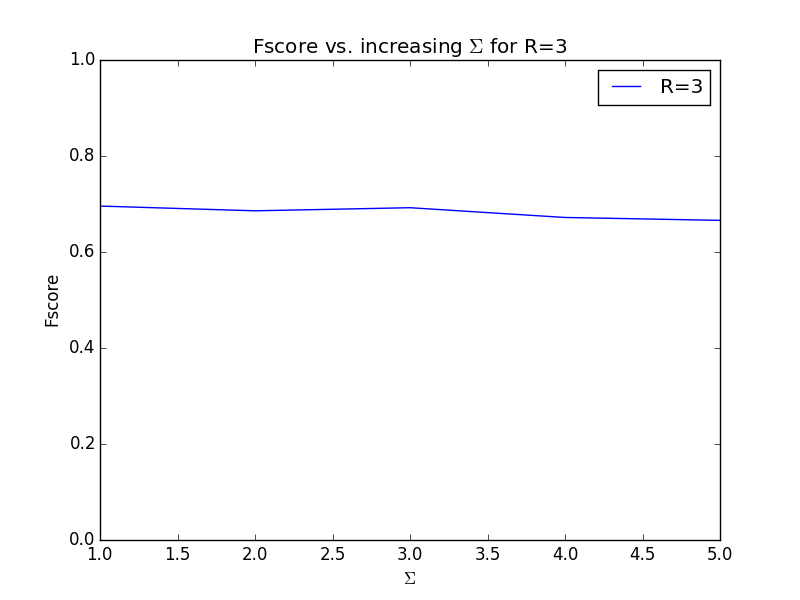
\includegraphics[width=1.0\textwidth]{6222-fscore_sigma_for_R3}
\caption{Fscore results for increasing $\Sigma$ at constant $R=3$}
\label{fig:fscore_r3}
\end{figure}

Holding R constant, the Fscore does not vary significantly with increasing Sigma, as shown in Figure~\ref{fig:fscore_r3}. This indicates that the smoothing of the GFP in 2D has little effect on zMod and, in turn, on zEdge.
